\documentclass{article}

\usepackage{amsmath}
\usepackage{amssymb}
\usepackage{parskip}
\usepackage{fullpage}
\usepackage{hyperref}
\usepackage{tikz}
\usepackage{url}
\usepackage{subfig}
\usepackage[backend=bibtex]{biblatex}

\usepackage{bettelini}

\hypersetup{
    colorlinks=true,
    linkcolor=black,
    urlcolor=blue,
    pdftitle={Improved bead sort using the Fourier Transform},
    pdfpagemode=FullScreen,
}

\addbibresource{./references.bib}

\title{Improved bead sort using the Fourier Transform}
\author{Paolo Bettelini}
\date{\today}

\begin{document}

\maketitle

\section{Introduction}

\subsection{Abstract}

Bead sort has always been an interesting, but useless, sorting algorithm
for integers. It is able to sort numbers without ever directly comparing them.
This paper presents my attempt to make it possibly more efficient
for software when sorting large arrays of numbers.
The resulting algorithm is efficient when sorting a large array of small integers,
preferably with few distinct elements.

\subsection{Bead sort}

\textit{Bead sort}\cite{beadsort} or \textit{gravity sort}
is a natural sorting algorithm.
This algorithm is primarily used to sort
integers, but can be extended to sort the rationals.

The basic idea is to represent the unsorted integers
in a matrix (\ref{fig:a}), where each columns has \(n\) beads.
We then shift every bead to the right side of the matrix
until they collide with another bead,
as if they were affected by gravity.
The final step is to count the elements in each columns,
forming the final ordered sequence (\ref{fig:b}).

\begin{figure}[h]
    \centering
  
    \subfloat[Unsorted beads]{
        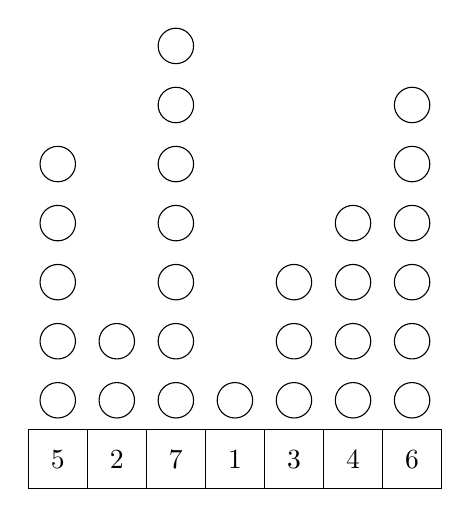
\begin{tikzpicture}[scale=0.75]
            % Draw the array
            \foreach \i/\n in {0/5, 1/2, 2/7, 3/1, 4/3, 5/4, 6/6} {
                \draw (\i,0) rectangle ++(1,1);
                \node at (\i+0.5, 0.5) {\n};
            }
            
            % Beads
            \foreach \i/\n in {0/5, 1/2, 2/7, 3/1, 4/3, 5/4, 6/6} {
                \pgfmathsetmacro{\beads}{\n}
                \foreach \j in {1,...,\beads} {
                \draw (\i+0.5, \j+0.5) circle (0.3cm);
                }
            }
        \end{tikzpicture}
        \label{fig:a}
    }
    \quad\(\longrightarrow\)\quad
    \subfloat[Sorted beads]{
        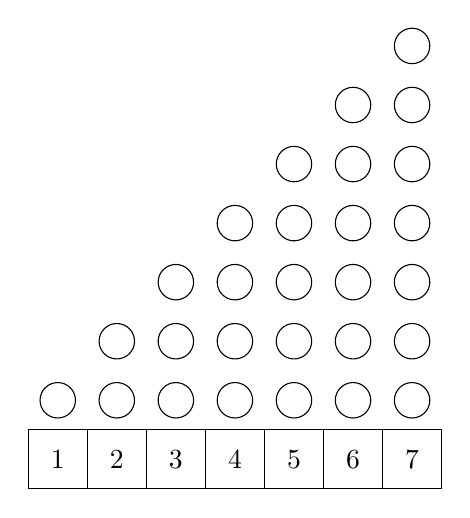
\begin{tikzpicture}[scale=0.75]
            % Draw the array
            \foreach \i/\n in {0/1, 1/2, 2/3, 3/4, 4/5, 5/6, 6/7} {
                \draw (\i,0) rectangle ++(1,1);
                \node at (\i+0.5, 0.5) {\n};
            }
            
            % Beads
            \foreach \i/\n in {0/1, 1/2, 2/3, 3/4, 4/5, 5/6, 6/7} {
                \pgfmathsetmacro{\beads}{\n}
                \foreach \j in {1,...,\beads} {
                \draw (\i+0.5, \j+0.5) circle (0.3cm);
                }
            }
        \end{tikzpicture}
        \label{fig:b}
    }
  
    \caption{Beads matrix for \(S = 5,2,7,1,3,4,6\)}
    \label{fig:both}
\end{figure}

The time complexity of this algorithm ranges from \(O(1)\)
to \(O(P)\) where \(P=\sum S_k\).

\pagebreak

\section{Algorithm}

\subsection{Core idea}

My idea is to represents the beads matrix as a
sum of sine functions. Each frequency represents a row,
and its amplitude the amount of elements in it.

For example

\begin{minipage}{0.3\textwidth}
    \begin{flushright}        
    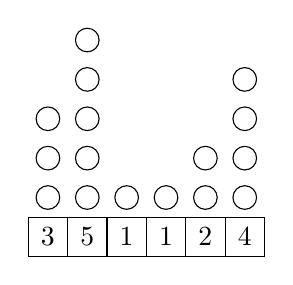
\begin{tikzpicture}[scale=0.5]
        % Draw the array
        \foreach \i/\n in {0/3, 1/5, 2/1, 3/1, 4/2, 5/4} {
            \draw (\i,0) rectangle ++(1,1);
            \node at (\i+0.5, 0.5) {\n};
        }
        
        % Beads
        \foreach \i/\n in {0/3, 1/5, 2/1, 3/1, 4/2, 5/4} {
            \pgfmathsetmacro{\beads}{\n}
            \foreach \j in {1,...,\beads} {
            \draw (\i+0.5, \j+0.5) circle (0.3cm);
            }
        }
    \end{tikzpicture}
    \end{flushright}
\end{minipage}
\begin{minipage}{0.5\textwidth}
    \[
        6\sin(t) + 4\sin(2t) + 3\sin(3t) + 2\sin(4t)+\sin(5t)
    \]
\end{minipage}

By using the Fourier Transform on the function representing the matrix
we can retrieve the amplitudes of the different frequencies
and construct the final beads matrix.

\subsection{Implementation}

Given a sequence of unordered natural numbers
\[
    S=\{n_k\},
    \quad
    0 < k \leq N
\]
we want to find a sequence
\[
    \hat{S}=\{m_l\},
    \quad
    0 < l \leq N
\]
which is the ordered version of \(S\).

We define a time-dependent function \(X(t)\)
\[
    X(t)=
    \sum_{k=1}^{|S|}
    \sum_{f=1}^{n_k}
    \sin(ft)
\]
By applying the Fourier Transform we get a frequency-dependent function
\[
    \hat{X}(\xi)=\mathcal{F}\{X(t)\}
\]

For all \(\xi \in \mathbb{N}\), the frequencies given by
\(|\hat{X}(\xi)|\) are integers, and they follow the property
\(|\hat{X}(\xi)| \geq |\hat{X}(\xi+1)|\).
In order to retrieve the ordered elements, we can gradually increase
the frequency \(\xi\) by \(1\) by starting at \(\xi=1\). \\
Let \(k=|\hat{X}(\xi)| - |\hat{X}(\xi+1)|\). Whenever \(k \neq 0\)
we consider \(\xi\) to be the next elements in the sequence of ordered
integers. The element \(\xi\) will be the next in the ordered sequence,
and it will appear \(k\) many times.
Repeat this process until all numbers have been extracted
\((\xi = \text{max}(S))\).

\pagebreak

\subsection{Computation}

\subsubsection{Complexity of \(X(t)\)}

The function \(X(t)\) has space complexity \(O(1)\).
It also has time complexity \(O(N\cdot P)\) where
\(P=\sum S_k\).
We can reduce the latter by noting that \(X(t)\) contains
a geometric series.

\begin{align*}
    \sum_{f=1}^{n_k} \sin(ft) 
    &= \Im \sum_{f=1}^{n_k} e^{ift} \\
    &= \Im \left( e^{it} \frac{e^{itn_k}-1}{e^{it}-1} \right) \\
    &= \Im \left( e^{it} \frac{e^{in_kt/2}(e^{in_kt/2} - e^{-in_kt/2})}
        {e^{it/2}(e^{it/2} - e^{-it/2})} \right) \\
    &= \Im \left( e^{it} \frac{e^{in_kt/2}(2i\sin(n_kt/2))}
        {e^{it} (2i\sin(t/2))} \right) \\
    &= \Im \left( e^{i(n_k+1)t/2} \frac{\sin(n_k t/2)}{\sin(t/2)} \right) \\
    &= \Im \left(
            ( \cos((n_k+1)t/2) + i\sin((n_k+1)t/2)) \frac{\sin(n_k t/2)}{\sin(t/2)}
        \right) \\
    &= \frac{\sin(n_k t/2)}{\sin(t/2)} \sin((n_k+1)t/2)
\end{align*}

Thus,
\[
    X(t) = \sum_{k=1}^{|S|} \frac{\sin(n_k t/2)}{\sin(t/2)} \sin((n_k+1)t/2)
\]
The time complexity of \(X(t)\) is now \(O(N)\).

\subsubsection{Complexity of \(\hat{X}(\xi)\)}

The Fourier Transform of \(X(t)\) is given by
\begin{align*}
    \hat{X}(\xi) &=
    \frac{1}{\text{max}-\text{min}}
    \integral[\text{min}][\text{max}]
    [e^{-2\pi it\xi}X(t)] [t] \\
    &= \frac{1}{\text{max}-\text{min}}
    \integral[\text{min}][\text{max}]
    [e^{-2\pi it\xi}\sum_{k=1}^{|S|} \frac{\sin(n_k t/2)}{\sin(t/2)} \sin((n_k+1)t/2)]
    [t]
    \\ 
\end{align*}

Since \(|S|\) is finite we can apply an
interchange of summation and integration
\[
    \hat{X}(\xi) =
    \frac{1}{\text{max}-\text{min}}
    \sum_{k=1}^{|S|}
    \,
    \integral[\text{min}][\text{max}]
    [\frac{\sin(n_k t/2)}{\sin(t/2)} \sin((n_k+1)t/2)e^{-2\pi it\xi}]
    [t]
\]

If \(\hat{X}(\xi)\) has a closed-form,
then its time and space complexities are the ones of \(X(t)\),
which are \(O(N)\) and \(O(1)\) respectively.
Alternatively, one may use the FFT algorithm,
which has time and space complexities \(O(N \log(N))\).

\subsubsection{Complexity of \(m_l\)}

The computation of \(m_l\) requires a scan
of the frequencies given by \(|\hat{X}(\xi)|\).
The amount of frequencies to consider is equal to the maximum
integer in the input.
Since the amplitude of the frequencies are ordered it may be optimized
using a binary search, giving a time complexity of \(O(Q)\)
where \(Q\) is the maximum integer.

The space complexity of this operation is always \(O(1)\).

\subsection{Total space complexity}

If a closed-form for \(\hat{X}(\xi)\) is found,
the total space complexity of the algorithm is \(O(1)\).

\section{Conclusion}

The Fourier transform is able to directly encode the data of the beads matrix
into a function efficiently. As the magnitude of the numbers to sort
increase, the efficiency of the algorithm drops. However, one may note
that multiple integers that are equal
will collapse in the same point of \(\hat{X}(\xi)\),
meaning that equal integers will not add complexity to the retrieval
of the elements from \(\hat{X}(\xi)\). Thus,
this algorithm is efficient for sorting large arrays of small integers
with few distinct elements.

\nocite{*} % cite all entries

\end{document}
